\chapter{Introduction}

% Mars entry problem - mission requirements and future stuff

% State of practice - MSL/M2020

% Covariance reduction based entry guidance - also discussion of sensivity based approaches and comparison work. Also terminology: robust OCP versus optim under unc versus...

% Introduction to my approach? 
% State the specific objectives of my research 

NASA has successfully landed five rovers on Mars to date, including the Mars 2020 rover Perseverance. Each of these missions chose low elevation targets between -1 and -4 km relative to the Mars areoid surface, commonly referred to as MOLA, after the instrument that was used to map Mars' topography. The thin Martian atmosphere makes aerodynamic deceleration ineffective except at lower altitudes where the atmosphere is denser. Coupled with the increasing entry mass required to deliver larger, more capable rovers to the surface, this makes high elevation landing on Mars a challenging problem. Nevertheless, targets above 0 km MOLA, like Terra Sirenum in the Southern Highlands, are motivated by scientific interest \cite{MarsWater}. In order for descent and landing operations to have sufficient timeline margin \cite{BraunMarsEDL,MSL_EDL2} when targeting such elevations, the entry phase must be terminated at a sufficiently high altitude.
%The entry phase may be terminated at a fixed velocity \cite{MSL_EDL2}, at a fixed downrange distance \cite{TriggerComparison2020}, or by a more complex function of the vehicle state \cite{LuAdaptiveEDL}. 
%Increasing altitude at a terminal entry state allows the vehicle to target landing sites at higher elevations, which are motivated by reasons of scientific interest, by increasing the time available for subsequent descent and landing operations, which is particularly important in high ballistic coefficient vehicles. 
In addition to terminal entry altitude, guidance designers must also consider additional objectives, such as reducing the size of the landing footprint. Often these multiple objectives are competing, as for example was the case on the Mars Science Laboratory (MSL) mission, where the entry guidance designers noted that targeting landing site elevations above -1 km MOLA would incur a larger landing ellipse \cite{MSL_EDL2}. 
Future missions, including sample return \cite{MSR} and manned, will place even greater emphasis on robust performance than the current generation, such as pinpoint landing requirements \cite{EvolvableMars}. 

%The state-of-the-practice for Mars entry guidance is represented by Mars 2020, which inherited its entry guidance architecture from MSL \cite{M2020_EDL}. 
%One change from MSL is that Mars 2020 initiated parachute deployment based on a range trigger rather than a velocity trigger \cite{TriggerComparison2020}. 
%MSL and Mars 2020 both utilized the entry terminal point controller (ETPC) \cite{MSL_EDL, M2020_EDL}, a modified version of the Apollo second phase guidance \cite{MSL_EDL2}.
The state-of-the-practice for Mars entry guidance, used on MSL and Mars 2020, is a modified version of the Apollo second phase guidance \cite{MSL_EDL2} called the entry terminal point controller (ETPC). 
The three phases of the ETPC are prebank, range control, and heading alignment. In the prebank phase, there is no guidance, but the vehicle is rotated to the expected initial bank angle for the start of the range control phase.
Range control begins when the vehicle-sensed drag acceleration exceeds a threshold value, and steers the vehicle to the correct downrange distance. This range control affects the longitudinal motion; separate lateral guidance operates during range control to command bank reversals when a measure of the crossrange to the target exceeds the deadband threshold, which is a quadratic function of velocity. At a specified velocity, the guidance switches from range control to heading alignment, during which the bank angle is commanded to reduce the crossrange error.

%TODO: Discuss possibility to handoff to SRP or something other than HeadingAlign/Parameter

The guidance design method used on these latest Mars entry vehicles \cite{MSL_EDL2,M2020_EDL} can be divided into two steps. The first step is to design a reference bank profile and compute the corresponding reference trajectory via open-loop simulation. The reference bank angle profile is specified by a small number of parameters, a modification from the original Apollo algorithm, which assumed a constant bank angle reference profile. This change allows for more flexibility in trajectory design, including enabling higher parachute deploy altitudes \cite{MSL_EDL2}.
In the second step, closed-loop performance using the reference trajectory and bank angle is evaluated under off-nominal conditions. A number of stress trajectories are simulated in closed-loop using the reference trajectory, ETPC gains, and heading alignment guidance to estimate off-nominal performance prior to Monte Carlo simulation \cite{MSL_EDL2}. The results are judged based on the vehicle state at parachute deployment. The free parameters of the guidance algorithm, including the overcontrol gain and heading alignment gain, are then tuned until the performance is satisfactory. If the necessary performance cannot be achieved through tuning, the reference trajectory is changed and the process is repeated. 

In this dissertation, we present an entry guidance law and the method for designing it. Compared with MSL and Mars 2020, the entry guidance objectives are the same, but the means of achieving the objectives and the design method are different. Like the MSL range controller, our guidance law modulates the vertical lift via the bank angle using reference-trajectory-based feedback control to reduce range and altitude dispersions and achieve high altitude, at the initial point of terminal descent which is the point of parachute deployment in the case of MSL and Mars 2020.  The differences in our approach are: (1) to minimize range and altitude dispersions and achieve high altitude, the reference trajectory and bank angle are solutions of a multi-objective robust optimal control problem for the closed-loop dynamics, (2) to address robustness, the state variables and uncertain parameters in the entry dynamics are treated as random variables, using the unscented transformation to approximate their means and variances, and state the performance index in terms of these statistics, (3) rather than a reference bank angle profile determined by a few parameters, a more general piecewise constant reference bank angle profile is considered, and (4) our feedback control law is a constant matrix multiplying the state vector. 
With this design approach, we aim to achieve better performance and avoid the many iterations of the two-step approach, involving 100s or 1,000s of reference trajectories \cite{MSL_EDL2}, used for MSL and Mars 2020. Monte Carlo simulation is only used post-design to validate and further characterize the guidance performance.
%TODO: Remove constant matrix claim above? Maybe not since we're optimizing the constants now 

Uncertainty is quantified using the unscented transformation (UT) \cite{UT1997}, allowing both means and standard deviations of key variables to be considered in the objective function of the optimal control problem, thereby formally addressing robust performance. The UT is a deterministic sampling-based method that propagates a set of sample points through the nonlinear dynamics and reconstructs the mean and covariance from the transformed samples. These sample trajectories allow us to estimate closed-loop guidance performance without Monte Carlo simulation, and thus serve a purpose similar to the MSL stress cases. The UT facilitates a computationally feasible approach to reference bank profile design accounting for uncertainty in a single step, rather than the MSL two-step process.

We demonstrate that, with a reformulation of the objective function, the robust optimal control problem can be solved using differential dynamic programming (DDP) \cite{DDP}, a shooting method originally devised to solve unconstrained nonlinear optimal control problems that has since seen numerous extensions, including to constrained problems \cite{DDP_ControlLimited,HDDP1,HDDP2,DDP_NonlinearConstraints,DDP_InteriorPoint}, and stochastic problems \cite{iLQG, DDP_Stochastic, ozaki_UT,ozaki2020tube}. 
Starting from the control-limited DDP algorithm \cite{DDP_ControlLimited}, we examine a iterated Linear-Quadratic-like simplification \cite{iLQG} that enables solution of large-scale optimal control problems. Next, we extend the algorithm to jointly optimize the static feedback gains along with the reference control.

% TODO: Talk about related work 
%Due to the interest in high elevation landings, guidance algorithms designed to maximize altitude at parachute deploy have been studied using optimal control theory 
%\cite{AltitudeOptimization,AltitudeOptimizationIndirect}. Reference \cite{GuangfeiDissertation} proposed an optimization-based onboard trajectory planning method based on a low-order parametrization designed to achieve high altitude at parachute deploy.
%Typically these papers consider predictive guidance and use parametrizations of the bank angle designed to yield high altitudes. 

% Refences with notes:
% AltitudeUnderUncertainty
% MarsEntryDesensitized % linearized but closed-loop with fixed gain. No consideration of saturation 
% EntryOUU % Does not use linearization, also doesnt solve in a conventional way, maybe remove?
% TrajectoryDesensitization % Desensitized like seywald and kumar, is it entry applied?
% EntryOUUThesis1 % Earth EDL, focuses on footprint computation, only considers open-loop in the reentry problem, and did not conduct monte carlo to confirm
% EntryOUUThesis2 % LQR, minimum control effort objective which stays away from the bounds, angle of attack as control variable. Does perform Monte Carlo(s) to validate improvement. 

Throughout this dissertation, we refer to optimal control formulations that weight a nominal (or mean) optimization objective with minimization of covariance terms as robust optimal control. The nomenclature in the literature also sometimes refer to such problems as uncertain optimal control \cite{PhelpsUncertainOCP}, optimal control under uncertainty. Due to the close relationship between the sensitivity matrix (also called the state transition matrix) and the covariance matrix, we also include desensitized optimal control \cite{Desensitized,TrajectoryDesensitization} under the umbrella of robust optimal control. 
Approaches to entry guidance based on robust optimal control have been studied in \cite{AltitudeUnderUncertainty, EntryOUUThesis1, EntryOUUThesis2, MarsEntryDesensitized, EntryOUU}. Reference~\cite{EntryOUUThesis1} explored the relationship between covariance reduction and sensitivity reduction, and ultimately recommended the covariance formulation for several reasons, including smaller problem size due to the symmetry of the covariance matrix, the ability to incorporate measurements, and simpler formulation and interpretation of variances compared to elements of the sensitivity matrix.

The works most closely related to our approach are Ref.~\cite{AltitudeUnderUncertainty}, where the objective was to maximize a function of the mean and standard deviation of altitude, and Ref.~\cite{MarsEntryDesensitized}, where the objective was to maximize terminal altitude while penalizing sensitivity terms related to variations in the initial state. Compared to Ref.~\cite{AltitudeUnderUncertainty}, our work differs by considering a multi-objective formulation that includes a downrange performance objective rather than strictly focusing on altitude, by considering closed-loop dynamics instead of open-loop, and by using the unscented transform instead of linear covariance propagation. Similarly, Ref.~\cite{MarsEntryDesensitized} also employed linear covariance propagation, but did consider closed-loop performance with fixed feedback gains. Their method made use of sensitivities, rather than statistics, in order to increase robustness to off-nominal situations. Additionally, a single penalty factor was applied to all terminal state sensitivities, including flight path angle. In contrast, we penalize only altitude and downrange deviations, and use a separate penalty factor for each component. An additional difference is that we consider parametric uncertainty in the equations of motion rather than solely uncertainty in the initial state. 

\begin{figure}[h!]
	\centering
	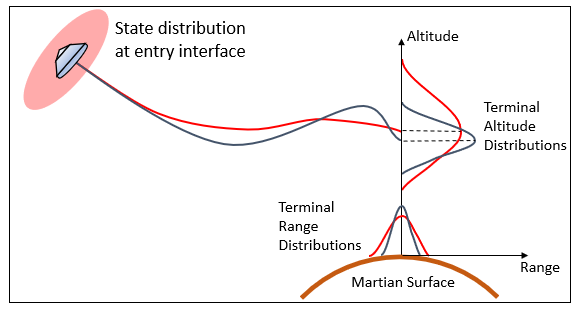
\includegraphics[width=1\textwidth]{Images/RobustTrajectoryOptimization}
	\caption{Comparison of UQ methods in an closed-loop scenario}
	\label{Fig:RobustTrajectoryOpt}
\end{figure}
%The specific objective of this dissertation are to design an entry guidance with the same computational complexity as the state-of-the-practice guidance algorithm while providing superior performance. 

%\section{Dissertation Organization}
This remainder of this dissertation is organized as follows: \\
chapter two discusses the dynamics and models used to describe entry trajectories\\
chapter three describes the entry guidance problem, especially target condition(s)\\
chapter four outlines the guidance strategy, including posing the problem as a ROCP. Gain optimization (or selection) as well. \\
chapter five gives an algorithm based on constrained DDP/SLQ to solve the ROCP; Also UQ and reformulations; demonstration of open-loop vs closed loop necessity of UT \\
chapter six presents the assessment conditions (simulation details, Monte Carlo) Maybe UT-alpha choice should be discussed here?\\
chapter seven presents an assessment of the guidance algorithm. Choice of alpha parameter. Problems with joint optimization as well (UT cov almost zero but MC cov bad) \\
chapter eight concludes the dissertation \\

chapter details two extensions to the DDP algorithm - an augmented lagrangian method for enforcing terminal constraints and a method for optimizing (constant) parameters, such as the feedback gains (lateral corridor params? probably not due to differentiable req) and the initial flight path angle. The gain optimization in particular is important because of the issue with joint optimization of time-varying gains. 

%%% Local Variables: ***
%%% mode: latex ***
%%% TeX-master: "thesis.tex" ***
%%% End: ***
